\documentclass[12pt]{article}

\usepackage{styles/log-style}

\begin{document}
\begin{titlepage}
\begin{center}
\bfseries

{\Large Московский Авиационный Институт\\ (национальный исследовательский университет)}

\vspace{36pt}

\large Институт информационных технологий и прикладной математики

\vspace{36pt}

\large Кафедра вычислительной математики и программирования

\vspace{48pt}

Журнал по исследовательской практике (индивидуальный план)

\end{center}

\vspace{120pt}

\begin{flushleft}
\begin{tabular}{|r|l|}
\hline
Студенты & Группа \\
\hline
Артемьев Дмитрий Иванович & М8О-406Б-18 \\
\hline
Белоусов Егор Владимирович & М8О-207Б-20 \\
\hline
Инютин Максим Андреевич & М8О-307Б-19 \\
\hline
Команда: & MAI \#2 Artemiev, Belousov, Inyutin \\
\hline
\end{tabular}
\end{flushleft}

\vspace*{\fill}

\begin{center}
\bfseries
Москва, \the\year
\end{center}
\end{titlepage}

\pagebreak

\subsection*{Сводная таблица за осень \the\year}
\resizebox{\columnwidth}{!}{
\begin{tabular}{|c|c|c|c|c|c|}
\hline
Дата & Название & Время & Место проведения & Решенные задачи & Дорешанные задачи \\
\hline
12.09.2021 & Grand Prix of Dolgoprudny & 11:00-16:00 & Дистанционно & G, H & D, I \\
\hline
19.09.2021 & Grand Prix of IMO & 11:00-16:00 & Дистанционно & A, E, H, N & F \\
\hline
10.10.2021 & XXII Открытая Всесибирская олимпиада & 10:00-15:00 & Дистанционно & 1, 3 & - \\
\hline
17.10.2021 & ICPC training MAI 21-22 & 11:00-16:00 & Дистанционно & A, D, F & G, H \\
\hline
24.10.2021 & Grand Prix of Korea & 11:00-16:00 & Дистанционно & H, G & C \\
\hline
07.11.2021 & Grand Prix of Siberia & 11:00-16:00 & Дистанционно & 1, 3, 5, 8 & - \\
\hline
14.11.2021 & Grand Prix of EDG & 11:00-16:00 & Дистанционно & A, D, E, G, I & B, F, K \\
\hline
21.11.2021 & RuCode 4.0 Div A-B Champoinship & 11:00-16:00 & Дистанционно & B, K & D \\
\hline
22.11.2021 & Div A + B Contest 1 & 09:00-14:00 & Дистанционно & C, D, H, L & F, J, K \\
\hline
26.11.2021 & Div A Contest 4: The Korean Contest & 09:00-14:00 & Дистанционно & B, C, L & D, G \\
\hline
12.12.2021 & Grand Prix of Nanjing & 11:00-16:00 & Дистанционно & A, C, H, M & - \\
\hline
19.12.2021 & Moscow Regional Contest & 11:00-16:00 & Дистанционно & A, D, E, F, G, H, N & - \\
\hline
\end{tabular}
}

\subsection*{Явка на контесты}
\resizebox{\columnwidth}{!}{
\begin{tabular}{|c|c|c|}
\hline
Дата & Название & Присутствующие \\
\hline
12.09.2021 & Grand Prix of Dolgoprudny & Артемьев, Белоусов, Инютин \\
\hline
19.09.2021 & Grand Prix of IMO & Артемьев, Белоусов, Инютин \\
\hline
10.10.2021 & XXII Открытая Всесибирская олимпиада & Артемьев, Белоусов, Инютин \\
\hline
17.10.2021 & ICPC training MAI 21-22 & Артемьев, Белоусов, Инютин \\
\hline
24.10.2021 & Grand Prix of Korea & Артемьев, Белоусов, Инютин \\
\hline
07.11.2021 & Grand Prix of Siberia & Артемьев, Белоусов, Инютин \\
\hline
14.11.2021 & Grand Prix of EDG & Артемьев, Белоусов, Инютин \\
\hline
21.11.2021 & RuCode 4.0 Div A-B Champoinship & Артемьев, Белоусов, Инютин \\
\hline
22.11.2021 & Div A + B Contest 1 & Артемьев, Белоусов, Инютин \\
\hline
26.11.2021 & Div A Contest 4: The Korean Contest & Артемьев, Белоусов, Инютин \\
\hline
12.12.2021 & Grand Prix of Nanjing & Артемьев, Белоусов, Инютин \\
\hline
19.12.2021 & Moscow Regional Contest & Артемьев, Белоусов, Инютин \\
\hline
\end{tabular}
}

\pagebreak

\includepdf[pages=10, scale=0.75, pagecommand=\subsection*{Grand Prix of Dolgoprudny 12.09.2021}]{statements/210830.pdf}
\subsubsection*{Идея}
Очевидно, что нужно всегда брать грани монет, которые присутствуют у оппонентов, то есть при наличии только одной монеты со значениями $1$ и $2$ не имеет смысла брать номинал $3$ на одну из граней нашей монеты, так как можно взять $2$ и потратить меньше денег. Пока мы не взяли ни одной грани полагаем, что наше математическое ожидание равняется $bad = -\sum_{i}x_i$, пусть тогда мы взяли на одну из сторон монеты $a'$, а на другую $b'$, тогда наше математическое ожидание равняется $E(a',b') = \sum_{i : a_i \leqslant a'}(\frac{x_i}{2}) + \sum_{i : b_i \leqslant a'}(\frac{x_i}{2}) + \sum_{i : a_i \leqslant b'}(\frac{x_i}{2}) + \sum_{i : b_i \leqslant b'}(\frac{x_i}{2}) + bad - a' \cdot b'$. Закинем все значения $a_i$ и $b_i$ в массив $z$ с коэффициентами $\frac{1}{2}$, отсортируем, посчитаем $pref_i = \sum_{j = 0}^{i - 1}z_i$. Упростим нашу сумму для подсчета математического ожидания: $E(a',b') = pref_{i'} + pref_{j'} + bad - a \cdot b$, где $i' : z_{i'} = a'$ и $j' : z_{j'} = b'$. В таком случае мы можем посчитать ответ за $O(n ^ 2 + n \cdot \log{n}) \approx O(n ^ 2)$ перебрав индексы в $z$. Улучшим решение до $O(n \cdot \log{n})$. Пусть мы уже выбрали $a'$, тогда мы хотим выбрать $b'$ такое, что $E(a', b') \rightarrow max$. Т.е. $E(a') = max_{b' \leqslant a'}(a'\cdot b' + pref_{j'}) + bad + pref_{i'}$. Заметим, что $a'\cdot b' + pref_{j'}$ при фиксированной $a'$ является прямой с $k = b'$ и $b = pref_{j'}$. В таком случае можно воспользоваться \textit{Convex hull trick}. Мы будем хранить множество прямых слева направо, так как угол наклона растет, то новую прямую мы будем добавлять справа, а также $a'$ тоже растет, поэтому мы сможем быстро узнавать максимум. Этот прием работает амортизованно за $O(n)$. Итоговая сложность: $O(n + n \cdot \log{n}) \approx O(n \cdot \log{n})$.
\subsubsection*{Исходный код}
\lstinputlisting{src/gp_dolgop_g.cpp}
\subsubsection*{Положение команды}
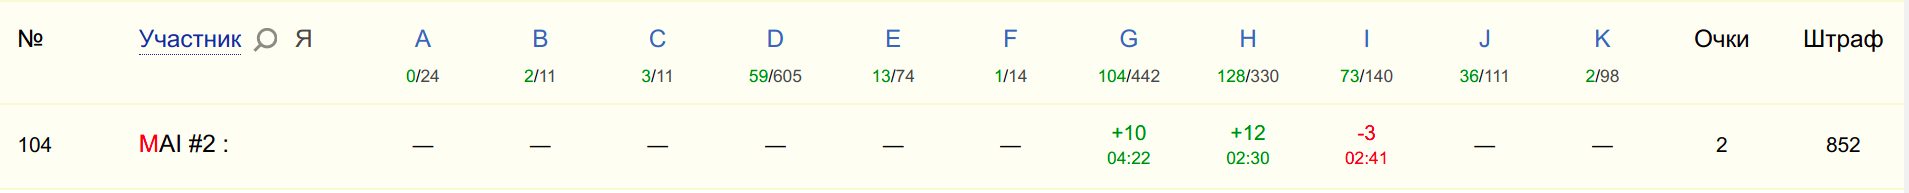
\includegraphics[scale=0.25]{images/gp_dolgop.png}\newline\noindent
\pagebreak

\includepdf[pages={11}, scale=0.75, pagecommand=\subsection*{Grand Prix of IMO 19.09.2021}]{statements/day3.en.pdf}
\subsubsection*{Идея}
Как известно, задача поиска Гамильтонова пути в графе является NP-полной. С помощью динамического программирования по подмножествам вычислительную сложность можно уменьшить с $O(n!)$ до $O(n ^ 2 \cdot 2 ^ n)$. Реализуем алгоритм, проверяющий какой-то граф на наличие Гамильтоновых путей между $K$ парами вершин $u$ и $v$.

Для маленьких $K$ нетрудно найти ответ. Для большего $K$ будем случайно генерировать графы и искать в них количество пар вершин $u$ и $v$ таких, что между ними есть Гамильтонов путь. Сгенерировав достаточно графов, можно увидеть закономерность, тогда решение становится полностью конструктивным, его асимптотика $O(K)$.

\subsubsection*{Исходный код}
\lstinputlisting{src/gp_imo_h.cpp}
\subsubsection*{Положение команды}
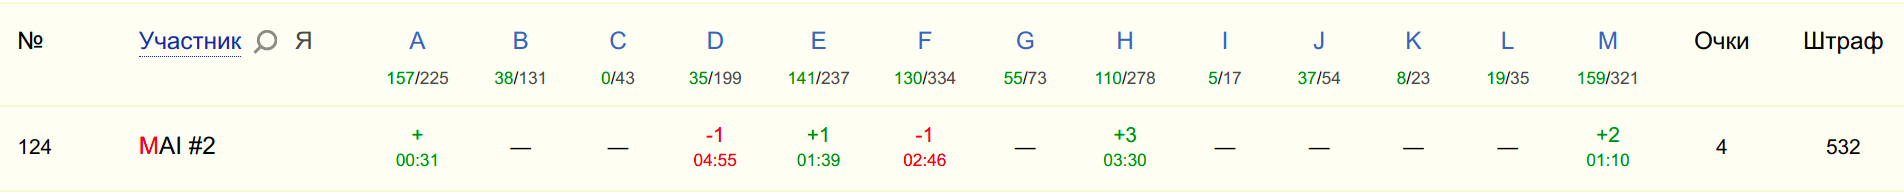
\includegraphics[scale=0.25]{images/gp_imo.png}\newline\noindent
\pagebreak

\includepdf[pages={2, 3}, scale=0.75, pagecommand=\subsection*{XXII Открытая Всесибирская олимпиада 10.10.2021}]{statements/sib.pdf}
\subsubsection*{Идея}
Для решения задачи требуется аккуратно реализовать проверку условий уровней конфликта. Если найденные моменты времени не противоречат условиям, то ответ <<Freytag>>, иначе <<Nein>>. Сложность решения $O(n)$.

\subsubsection*{Исходный код}
\lstinputlisting{src/sib_a.cpp}
\subsubsection*{Положение команды}
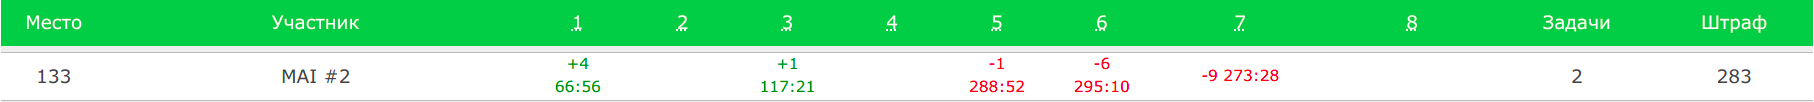
\includegraphics[scale=0.25]{images/sib.png}\newline\noindent
\pagebreak

\includepdf[pages={8, 9}, scale=0.75, pagecommand=\subsection*{ICPC training MAI 21-22 17.10.2021}]{statements/training1mai21.pdf}
\subsubsection*{Идея}
Для проверки подлинности таблицы составим наихудший и наилучший возможный рейтинг команды. Зная это, мы можем легко проверить, является ли часть таблицы верной. Асимптотика решения $O(n \cdot (k + m))$.

\subsubsection*{Исходный код}
\lstinputlisting{src/training1mai21_f.cpp}
\subsubsection*{Положение команды}
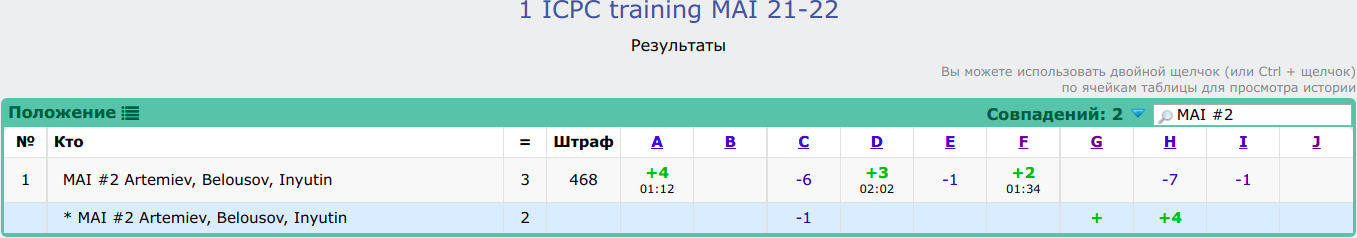
\includegraphics[scale=0.25]{images/training1mai21.png}\newline\noindent
\pagebreak

\includepdf[pages={12}, scale=0.75, pagecommand=\subsection*{Grand Prix of Korea 24.10.2021}]{statements/contest-24341-en.pdf}
\subsubsection*{Идея}
Давайте решим задачу для одного бита. Понятно, что решив такую задачу мы сможем с легкостью решить изначальную задачу ввиду того, что \textit{OR} одного бита не влияет на остальные.

Построим граф, вершины будут представлять собой регистры. Добавим ориентрированные ребра, ребро из $a$ в $b$ с весом $w$ будет обозначать, что $w$ команда будет присваивать $x_b = x_b | x_a$. Тогда нам потребуется найти минимальное время для каждой вершины, через которое произойдет замена бита $0$ на $1$. Это проблема легко решается с помощью алгоритма Дейкстры: просто запустим Дейкстру из всех таких регистров, в которых изначально стоит $1$, и немного поменяем метрику при пересчете расстояний.

Проделаем данный алгоритм для всех $8$ битов. В конце концов, для каждой вершины поставим $1$ в $i$-ом бите, если мы успеем его достичь быстрее чем за $t$ операций.

Итого решение работает за такую асимптотику $O(k \cdot l \cdot \log{n})$, где $k$ - это количество битов, в нашем случае $k = 8$.

\subsubsection*{Исходный код}
\lstinputlisting{src/gp_korea_j.cpp}
\subsubsection*{Положение команды}
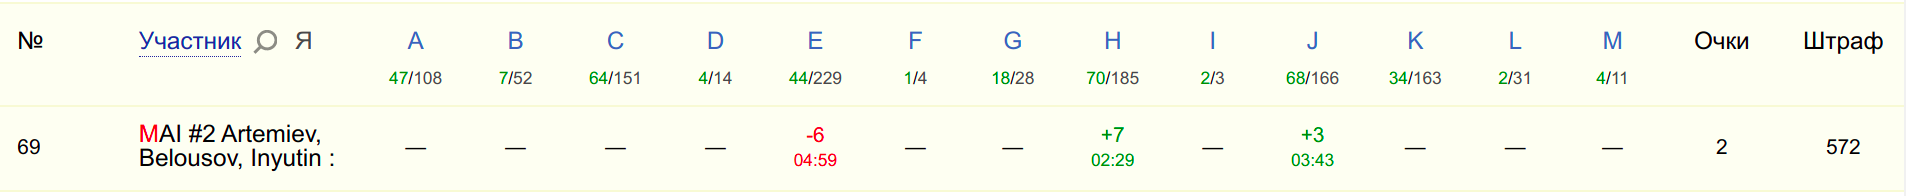
\includegraphics[scale=0.25]{images/gp_korea.png}\newline\noindent
\pagebreak

\includepdf[pages={5, 6}, scale=0.75, pagecommand=\subsection*{Grand Prix of Siberia 07.11.2021}]{statements/ocmgp5.ru.pdf}
\subsubsection*{Идея}
Основная сложность --- правильно реализовать систему штрафов в хоккее. Для этого каждую секунду игры. Если в какой-то момент времени на поле произошло событие, то его следует обработать согласно правилам игры. Для этого для каждого игрока обеих команд будем хранить тип штрафа и оставшееся время вне игры, постепенно уменьшая его. Остаётся проверять, сколько игроков на поле и увеличивать время для соответствующего состояния игры. Моделирование работает за константу, поэтому сложность решения $O(60 \cdot 60 \cdot 10 + n) \approx O(n)$.

\subsubsection*{Исходный код}
\lstinputlisting{src/gp_siberia_5.cpp}
\subsubsection*{Положение команды}
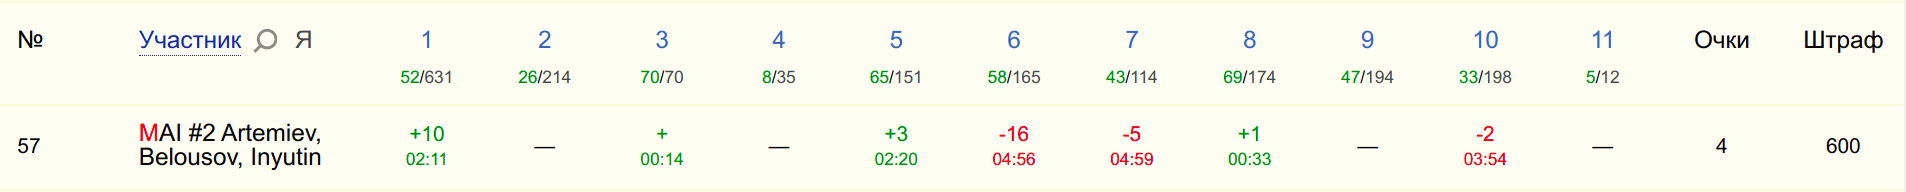
\includegraphics[scale=0.25]{images/gp_siberia.png}\newline\noindent
\pagebreak

\includepdf[pages=3, scale=0.75, pagecommand=\subsection*{Grand Prix of EDG 14.11.2021}]{statements/ocmgp6.en.pdf}
\subsubsection*{Идея}
Тривиальный случай, когда изменяется только одна цифра суммы, нам не очень интересен, так как изменяется всего две цифры во всех числах. Гораздо более сложный случай --- замена девяток на нули и нулей на девятки при изменении суммы. Заметим, что для какого-то префикса числа достаточно знать количество цифр <<0>> и <<9>>, чтобы корректно отвечать на запрос.

Используем струкуру данных, поддерживающую модификацию на отрезке для эффективного ответа на запрос и изменение. Во время контеста было реализовано решение с использованием Декартова дерева, которое не прошло по времени из-за большой константы. При дорешивании было реализовано решение, использующее дерево отрезков.

Сложность операций с деревом $O(\log{n})$. Асимптотика решения $O(n \cdot \log{n} + q \cdot \log{n})$.

\subsubsection*{Исходный код}
\lstinputlisting{src/gp_edg_b.cpp}
\subsubsection*{Положение команды}
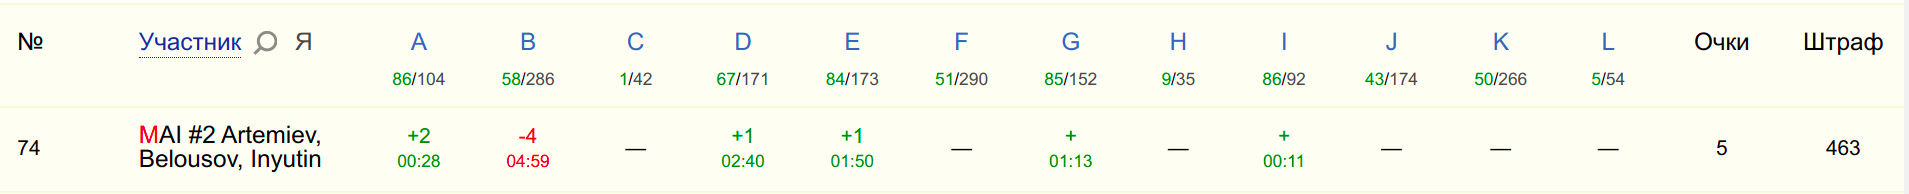
\includegraphics[scale=0.25]{images/gp_edg.png}\newline\noindent
\pagebreak

\includepdf[pages=2, scale=0.75, pagecommand=\subsection*{RuCode 4.0 Div A-B Champoinship 21.11.2021}]{statements/rucodeAB-ru.pdf}
\subsubsection*{Идея}
Решение задачи полностью конструктивное, полностью описано в программе. Самый сложный случай --- при нечётных ширине или высоте складов СберМаркета. Асимптотика $O(w \cdot h)$.
\subsubsection*{Исходный код}
\lstinputlisting{src/rucode_b.cpp}
\subsubsection*{Положение команды}
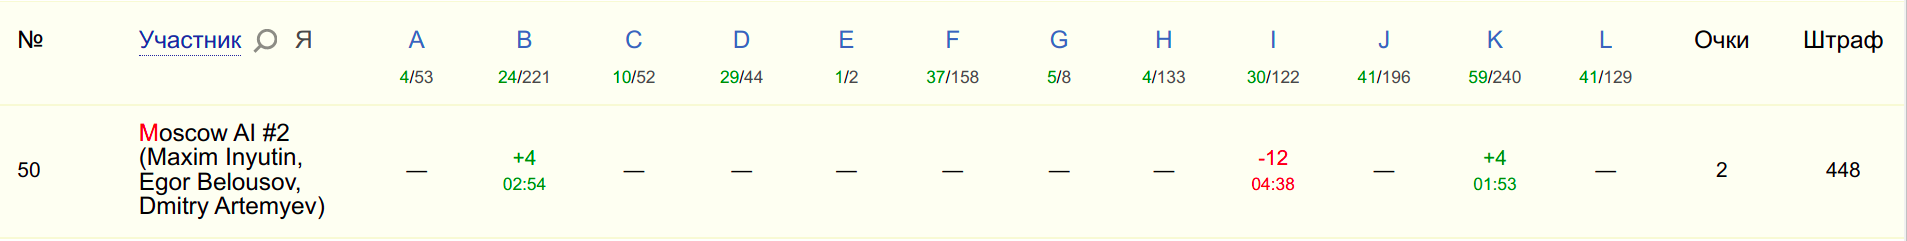
\includegraphics[scale=0.25]{images/rucode.png}\newline\noindent
\pagebreak

\includepdf[pages={14,15}, scale=0.75, pagecommand=\subsection*{Div A + B Contest 1 22.11.2021}]{statements/211122.en.pdf}
\subsubsection*{Идея}
Для решения задачи построим дерево отрезков на сумму чисел, стоящих на чётных и нечётных позициях для всего забора. Будет обновлять каждый фрагмент забора и выводить требуемую сумму. Так как суммарно обновлений в дереве будет не более $\sum a_i \leqslant 10 ^ 6$ и $n \leqslant 10 ^ 6$, то итоговая временная сложность решения $O(n \cdot \log{n})$.
\subsubsection*{Исходный код}
\lstinputlisting{src/mw1_f.cpp}
\subsubsection*{Положение команды}
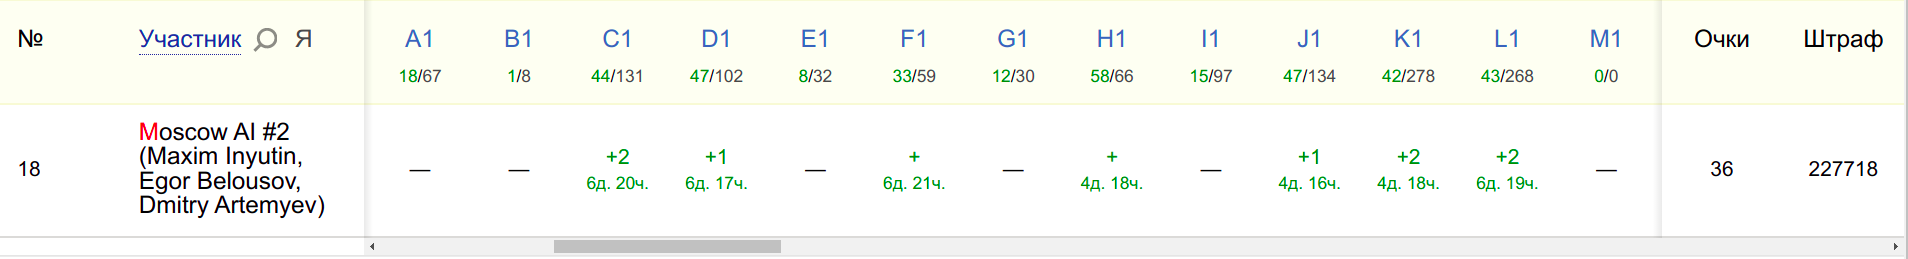
\includegraphics[scale=0.25]{images/mw1.png}\newline\noindent
\pagebreak

\includepdf[pages=21, scale=0.75, pagecommand=\subsection*{Div A Contest 4: The Korean Contest 26.11.2021}]{statements/211126.en.pdf}
\subsubsection*{Идея}
Используем \textit{std::bitset} для эффективного хранения чисел. Для каждого разряда и для каждой цифры хранится битовое множество позиций чисел из множества $A$. Добавление и удаление чисел из такой структуры очень простое и выполняется фактически за $O(1)$. Пространственная сложность такого хранения $O({{4 \cdot 9 \cdot n}\over{64}}) \approx O(n)$.

Зафиксируем два числа тройки. Выберем только те цифры, которые удовлетворяют условию тройки, добавим в ответ количество индексов чисел. Операция \textit{count} для \textit{std::bitset} выполняется за $O({n \over 64})$, поэтому временная сложность решения $O({{n ^ 3} \over 64})$.
\subsubsection*{Исходный код}
\lstinputlisting{src/mw4_l.cpp}
\subsubsection*{Положение команды}
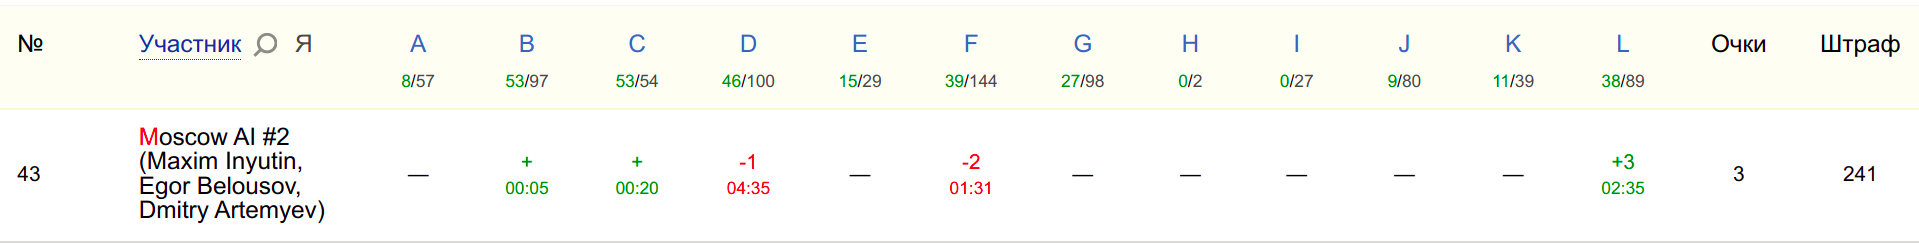
\includegraphics[scale=0.25]{images/mw4.png}\newline\noindent
\pagebreak

% Можно и другую задачу
\includepdf[pages={14,15}, scale=0.75, pagecommand=\subsection*{Grand Prix of Nanjing 12.12.2021}]{statements/ocmgp9.en.pdf}
\subsubsection*{Идея}
Решим сперва чуть более простую задачу, в которой бабочки улетают через 1 или 2 секунды. Возьмем вершину $1$ за корень дерева.
Пусть мы зашли в какую-то вершину и испугали всех смежных бабочек, тогда в вершины, где бабочки улетают через $1$ или $2$ секунды после испуга, мы, если хотим собрать бабочек, должны заходить сразу же, так как, если мы зайдем в другую вершину дерева, то нам придется потратить по крайней мере $3$ секунды.
Тогда пусть $dp_i$ обозначает максимальное кол-во бабочек, которые мы соберем, если начнем собирать в вершине $i$. Пересчет динамики таков: $dp_i = max_{j}\{\sum_{c \neq j}(dp_c - a_c) + dp_j\}$ где $j$ и $c$ являются детьми $i$ в дереве, с корнем в $1$.
Для того, чтобы пересчитать динамику в вершинах с $3$ секундами введем еще значение $dpvis_i$ --- сколько бабочек мы соберем, начиная с вершины $i$, если мы не возьмем бабочек в вершине $i$, а также во всех детях $i$, но возьмем бабочек во всех детях детей $i$. Пересчет достаточно прост: $dpvis_i$ = $\sum_{c}(dp[c] - a[c])$, где $c$ --- ребенок $i$. В конце концов пересчитаем динамику для $i$ дополнительно по вершинам с испугом в $3$ секунды: $dp_i = max_{j, k : j \neq k}\{\sum_{c \neq j, c \neq k}(dp_c - a_c) + dpvis_k + a_k + dp_j\}$, $j$ вершина с испугом в 3 секунды. Итого, используя поиск в глубину и предпосчитав суммы через префиксные суммы, можно решить данную задачу за $O(n)$
\subsubsection*{Исходный код}
\lstinputlisting{src/gp_nanjing_h.cpp}
\subsubsection*{Положение команды}
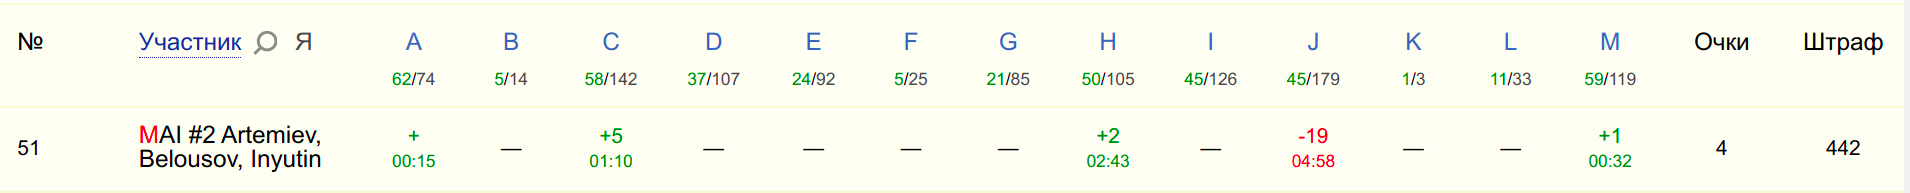
\includegraphics[scale=0.25]{images/gp_nanjing.png}\newline\noindent
\pagebreak

\includepdf[pages=7, scale=0.75, pagecommand=\subsection*{Moscow Regional Contest 19.12.2021}]{statements/contest-25256-en.pdf}
\subsubsection*{Идея}
Предпосчитаем $\gcd$ для первых $10000$ чисел. Видно, что для больших чисел почти всегда $\gcd$ его анаграм равен 1. Но есть и исключения, которые мы обработаем отдельно. Наиболее интересны числа, состоящие из чётных цифр и сумма цифр которых делится на три. При перестановке цифр в таком числе делимость на $3$ и $2$ не изменится. Сложность решения $O(t +k)$, где $k$ --- константа предподсчёта $k \approx 10 ^ 4 \cdot 4! \cdot 4 \cdot \log{10 ^ 4}$.
\subsubsection*{Исходный код}
\lstinputlisting{src/moscow_regional_e.cpp}
\subsubsection*{Положение команды}
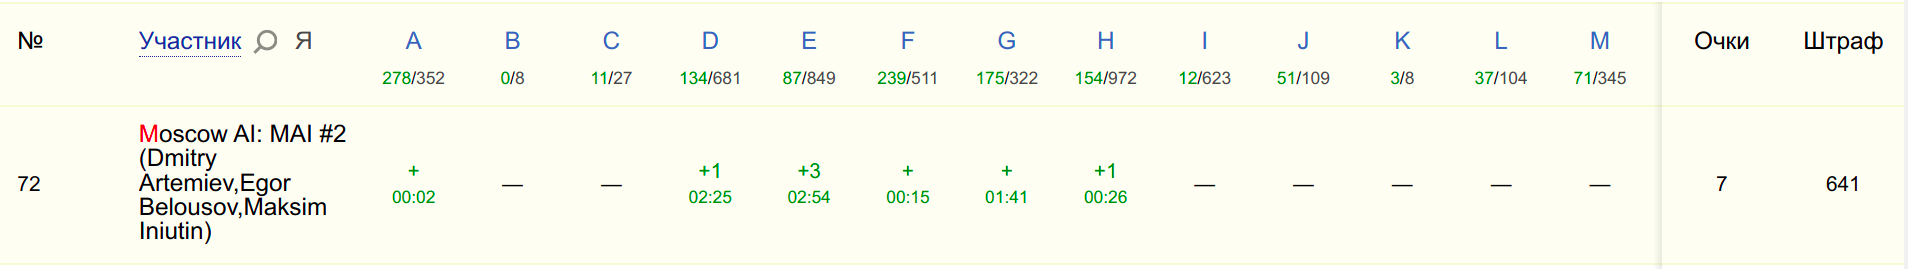
\includegraphics[scale=0.25]{images/moscow_regional.png}\newline\noindent
\pagebreak

\end{document}
